\documentclass[11pt]{article}

\usepackage[utf8]{inputenc}

\usepackage{geometry}
\geometry{a4paper}

\usepackage{graphicx}
 \graphicspath{ {.}{../img_einheiten/} }

\usepackage{array}
\usepackage{verbatim}

\usepackage{fancyhdr}
\pagestyle{fancy}
\renewcommand{\headrulewidth}{0pt}
\lhead{}\chead{}\rhead{}
\lfoot{}\cfoot{\thepage}\rfoot{}

\begin{document}

\subsection{Spielobjekte}

Spielobjekte werden unterteilt in:
\begin{description}
\item[Einheiten]\hfill \\
Hierzu z\"ahlen alle Einheiten welche vom Spieler, Gegner oder von einer neutralen Partei kontrolliert werden.
\item[Sonstige Objekte]\hfill \\
Hierzu z\"ahlen alle sonstigen Objekte im Spiel wie z.B. Elemente der Umgebung.
\end{description}

\subsubsection{Einheiten}
Es gibt Einheiten welche vom Spieler, Gegner und von einer neutralen Partei kontrolliert werden. Sie k\"onnen durch die Spielwelt bewegt werden, Zellteilung betreiben oder gegnerische Einheiten angreifen (siehe \textit{Optionen \& Aktionen}). Einheiten haben gewisse Eigenschaften, nicht jede Einheit hat jedoch alle Eigenschaften, z.B. k\"onnen manche nicht angreifen. Alle Eigenschaften von Einheiten sind in der \textit{Eigenschaftstabelle} aufgef\"uhrt:

\begin{tabular}{|r|l|}
\hline
Eigenschaft		& Beschreibung\\\hline\hline
Lebenspunkte	& Lebenspunkte einer Einheit von 1 (wenig) bis 10 (viel).\\
			& Wird u.a. im Kampf durch gegnerische Angrifssst\"arke gesenkt.\\
			& Erreichen sie den Nullpunkt ist die betroffene Einheit besiegt.\\\hline
Angriffsst\"arke	& Maßgebend f\"ur den Schaden von 1 (schwach) bis 10 (stark) den\\
			& eine Einheit im Kampf ausrichtet um dadurch die Lebenspunkte\\
			& anderer Einheiten zu senken.\\
			& Bei Viren gibt dieser Wert an wie schnell sie\\
			& eine Einheit verglichen mit deren Virenresistenz infizieren.\\\hline
Virenresistenz	& Von 1 (schwach) bis 10 (stark) gibt dieser Wert an wie resistent\\
			& eine Einheit gegen Viren ist. Einheiten welche vom Gegner\\
			& kontrolliert werden haben diese Eigenschaft nicht.\\
			& Dies ist maßgebend daf\"ur wielange ein Virus\\
			& verglichen mit seiner Angriffsst\"arke braucht um die betroffene\\
			& Einheit zu infizieren.\\\hline
Lebensdauer		& Gibt in Werten von 1 (kurz) bis 10 (lang) an wie lang,\\
			& gemessen in Zeit, eine Einheit im Spiel verbleibt bis sie durch\\
			& abgeloffene Lebensdauer besiegt wird.\\\hline
Geschwindigkeit	& In Werten von 1 (langsam) bis 10 (schnell) maßgebend f\"ur\\
			& die Geschwindigkeit einer Einheit beim Bewegen auf der Spielkarte\\\hline
Teilungsgeschwindigkeit	& Von 1 (langsam) bis 10 (schnell) gibt dieser Wert an wie lange\\
			& eine Zellteilung der betroffenen Einheit dauert. Bei Viren gibt\\
			& dies an wie lang die seine Verbreitung nach einer Zellinfektion\\
			& dauert da diese nicht normale Zellteilung anwenden k\"onnen.\\\hline
Stamm		& Spezielle Eigenschaft von Bakterien und Viren, sie gibt an welchem\\
			& Bakterien- bzw. Virenstamm jene Einheiten angeh\"oren.\\
			& Kann durch Zellteilung ver\"andert werden und ist maßgeblich\\
			& f\"ur die Bildung von Antigenen.\\\hline
Antigen		& Spezielle Eigenschaft von B-, T-, und Riesenfresszellen\\
			& sowie von Antik\"orpern.\\
			& Wird durch Besiegen gegnerischer Einheiten\\
			& gewonnen und gibt an gegen welchen Bakterien- bzw. Virenstamm\\
			& die Einheit ein Antigen produziert hat.\\
			& Ist maßgeblich f\"ur die spezifische Bek\"ampfung von Feinden.\\\hline
\multicolumn{2}{c}{}\\
\multicolumn{2}{c}{\textit{\large{Eigenschaftstabelle}}}\\
\end{tabular}
\newline\newline\newline
Im folgenden werden alle Einheiten in der \textit{Einheitentabelle} mit ihren entsprechenden Eigenschaften aufgef\"uhrt:

\begin{tabular}{|r|l|}
\hline
\multicolumn{2}{c}{Stammzelle}\\
\multicolumn{2}{c}{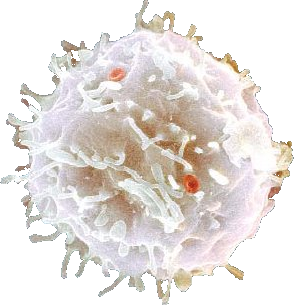
\includegraphics[width=2cm]{stemcellorig.png}}\\\hline\hline
Beschreibung:	& Eine Stammzelle ist eine vom Spieler kontrollierte Einheit.\\
			& In einem Level startet der Spieler zu Beginn immer\\
			& mit einer Stammzelle. Sie dient der Produktion von\\
			& anderen Stamm-, B-, T- und Riesenfresszellen\\
			& sowie von roten Blutk\"orperchen durch Zellteilung.\\
			& Die Zellteilung einer Stammzelle dauert\\
			& wesentlich k\"urzer als die anderer Einheiten im Gegenzug\\
			& kann sie nicht angreifen.\\\hline
Lebenspunkte	& 7\\\hline
Virenresistenz	& 6\\\hline
Lebensdauer		& 7\\\hline
Geschwindigkeit	& 2\\\hline
Teilungsgeschwindigkeit	& 7\\\hline
\end{tabular}

\begin{tabular}{|r|l|}
\hline
\multicolumn{2}{c}{B-Zelle}\\
\multicolumn{2}{c}{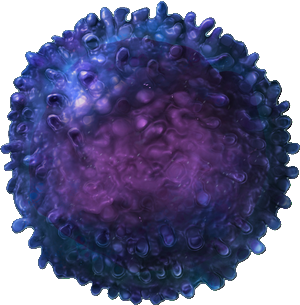
\includegraphics[width=2cm]{bcellorig.png}}\\\hline\hline
Beschreibung:	& Eine B-Zelle ist eine vom Spieler kontrollierte Einheit\\
			& und wird zur spezifischen Abwehr gez\"ahlt.\\
			& Erh\"alt die B-Zelle ein Antigen kann diese\\
			& Antik\"orper Einheiten produzieren.\\
			& Desweiteren kann die B-Zelle weitere B-Zellen Einheiten\\
			& durch Zellteilung produzieren, besitzt sie\\
			& dabei ein Antigen wir diese Eigenschaft an die\\
			& produzierten Einheiten weitergegeben.\\
			& Bei der Erstellung einer B-Zelle k\"onnen\\
			& bestimmte Eigenschaftswerte vergeben werden\\
			& welche an produzierte Antik\"orper weitergegeben\\
			& werden. Dies bestimmt welche Werte und um\\
			& wieviel Antik\"orper von feindlichen Einheiten verringern.\\
			& Diese Einheit kann nicht angreifen.\\\hline
Lebenspunkte	& 3\\\hline
Virenresistenz	& 3\\\hline
Lebensdauer		& 3\\\hline
Geschwindigkeit	& 4\\\hline
Teilungsgeschwindigkeit	& 2\\\hline
\end{tabular}

\begin{tabular}{|r|l|}
\hline
\multicolumn{2}{c}{T-Zelle}\\
\multicolumn{2}{c}{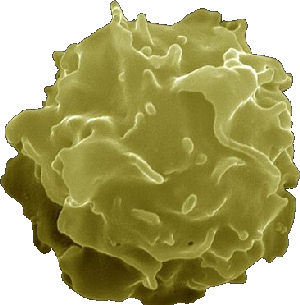
\includegraphics[width=2.0cm]{tcellorig.png}}\\\hline\hline
Beschreibung:	& Die T-Zelle ist eine vom Spieler kontrollierte\\
			& Einheit und wird zur spezifischen Abwehr\\
			& gez\"ahlt. Erh\"alt die T-Zelle ein\\
			& Antigen bekommt sie im Kampf gegen eine\\
			& Einheit welche vom Stamm des Antigens\\
			& eine Angrifsst\"arkebonus von 3.\\
			& Die T-Zelle ist in der Lage Viren, welche\\
			& Zellen infiziert haben anzugreifen und\\
			& diese, im Falle eines erfolgreichen\\
			& Kampfausgangs, zu befreien indem die\\
			& Virus Einheit vernichtet wird.\\
			& Die T-Zelle ist in der Lage weitere T-Zellen\\
			& Einheiten durch Zellteilung zu produzieren,\\
			& besitzt sie dabei ein  Antigen wird diese\\
			& Eigenschaft an die produzierten\\
			& Einheiten weitergegeben.\\
			& Die T-Zelle kann nicht auf normalem\\
			& Wege angreifen.\\\hline
Lebenspunkte	& 6\\\hline
Angriffsst\"arke	& 3 (+3 mit Antigenbonus)\\\hline
Virenresistenz	& 5\\\hline
Lebensdauer		& 4\\\hline
Geschwindigkeit	& 4\\\hline
Teilungsgeschwindigkeit	& 2\\\hline
\end{tabular}

\begin{tabular}{|r|l|}
\hline
\multicolumn{2}{c}{Riesenfresszelle}\\
\multicolumn{2}{c}{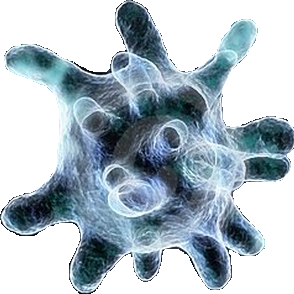
\includegraphics[width=2.0cm]{fresszelleorig.png}}\\\hline\hline
Beschreibung:	& Die Riesenfresszelle ist eine vom Spieler\\
			& kontrollierte Einheit und wird zur\\
			& unspezifischen Abwehr gez\"ahlt.\\
			& Sie ist f\"ur den Kampf sowie den\\
			& Gewinn von Antigenen konzipiert.\\
			& Im Gegensatz zur T-Zelle ist sie nicht\\
			& in der Lage von einem Virus befallene\\
			& Zellen anzugreifen um sie zu befreien.\\
			& Die Riesenfresszelle kann keine Zellteilung\\
			& anwenden. Besiegt sie eine feindliche\\
			& Einheit erh\"alt sie ein Antigen gegen\\
			& dessen Stamm. Dieses kann dann z.B.\\
			& an B- oder T-Zellen weitergegeben werden.\\\hline
Lebenspunkte	& 5\\\hline
Angriffsst\"arke	& 4\\\hline
Virenresistenz	& 3\\\hline
Lebensdauer		& 3\\\hline
Geschwindigkeit	& 5\\\hline
\end{tabular}

\begin{tabular}{|r|l|}
\hline
\multicolumn{2}{c}{Antik\"orper}\\\hline\hline
\multicolumn{2}{c}{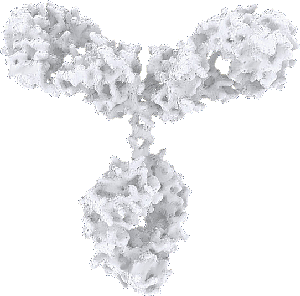
\includegraphics[width=2cm]{antikoerperorig.png}}\\\hline\hline
Beschreibung:	& Antik\"orper sind vom Spieler kontrollierte\\
			& Einheiten und werden zur spezifischen\\
			& Abwehr gez\"ahlt. Sie werden von\\
			& B-Zellen, welche Antigene besitzen,\\
			& produziert. Dabei \"ubernimmt\\
			& der Antik\"orper die Antigen Eigenschaft.\\
			& Er ist in der Lage feindliche Einheiten\\
			& vom Stamm seines Antigens zu befallen.\\
			& Dabei verringert der Antik\"orper die\\
			& Eigenschaften der feindlichen Einheit\\
			& um vorbestimmte Werte.\\
			& Diese Werte werden bei der Erstellung\\
			& durch die B-Zelle festgelegt.\\
			& Die Einheit kann nach einem Befall\\
			& nicht mehr vom Spieler kontrolliert werden.\\
			& Diese Einheit kann keine Zellteilung\\
			& anwenden und nicht auf normalem\\
			& Wege angreifen.\\\hline
Lebenspunkte	& 3\\\hline
Virenresistenz	& 2\\\hline
Lebensdauer		& 4\\\hline
Geschwindigkeit	& 7\\\hline
\end{tabular}

\begin{tabular}{|r|l|}
\hline
\multicolumn{2}{c}{Rote Blutk\"orperchen}\\\hline\hline
\multicolumn{2}{c}{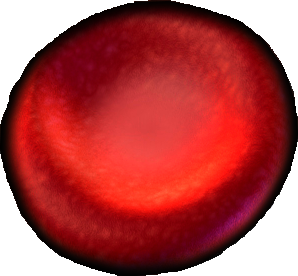
\includegraphics[width=2cm]{redbloodcella.png}\quad\quad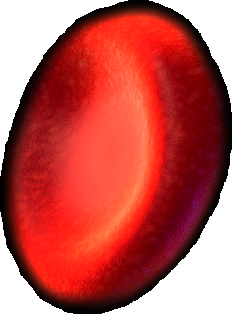
\includegraphics[width=2cm]{redbloodcellb.png}\quad\quad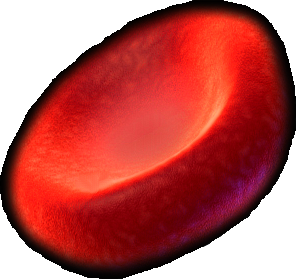
\includegraphics[width=2cm]{redbloodcellc.png}\quad\quad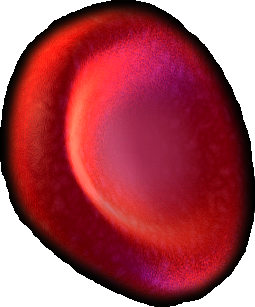
\includegraphics[width=2cm]{redbloodcelld.png}}\\\hline\hline
Beschreibung:	& Rote Blutk\"orperchen werden nicht vom\\
			& Spieler oder Gegner kontrolliert.\\
			& Sie geh\"oren der Fraktion des Spielers\\
			& an und k\"onnen von feindlichen\\
			& Einheiten angegriffen werden sowie\\
			& von deren Viren befallen werden.\\
			& Sie bewegen sich selbstst\"andig,\\
			& k\"onnen nicht angreifen oder\\
			& Zellteilung betreiben.\\
			& Gibt es zu wenig rote Blutk\"orperchen\\
			& verliert der Spieler.\\\hline
Lebenspunkte	& 3\\\hline
Virenresistenz	& 2\\\hline
Lebensdauer		& 4\\\hline
Geschwindigkeit	& 5\\\hline
\end{tabular}

\begin{tabular}{|r|l|}
\hline
\multicolumn{2}{c}{Bakterium}\\\hline\hline
\multicolumn{2}{c}{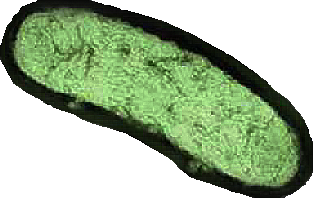
\includegraphics[width=2cm]{bakteriumorig.png}}\\\hline\hline
Beschreibung:	& Bakterien sind vom Gegner kontrollierte\\
			& Einheiten. Sie besitzen die  Eigenschaft\\
			& Stamm welche sie einem Stamm zuordnet.\\
			& Die Einheit ist in der Lage andere\\
			& Bakterien durch Zellteilung zu produzieren\\
			& wodurch ihr Stamm an diese weitergegeben\\
			& wird. Dabei kann es auch passieren,\\
			& dass die so produzierte Einheit einem\\
			& neuen Stamm angeh\"ort. Bakterien\\
			& k\"onnen Einheiten des Spielers angreifen.\\
			& Die Angriffsst\"arke von Bakterien gegen\\
			& andere Zellen ist je nach Zellenart\\
			& unterschiedlich und kann \"uber Mutation\\
			& spezialisiert werden.\\\hline
Lebenspunkte	& 5\\\hline
Angriffsst\"arke	& 4\\\hline
Lebensdauer		& 3\\\hline
Geschwindigkeit	& 5\\\hline
Teilungsgeschwindigkeit	& 3\\\hline
\end{tabular}

\begin{tabular}{|r|l|}
\hline
\multicolumn{2}{c}{Virus}\\\hline\hline
\multicolumn{2}{c}{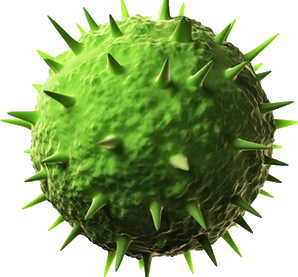
\includegraphics[width=2cm]{virusaorig.png}\quad\quad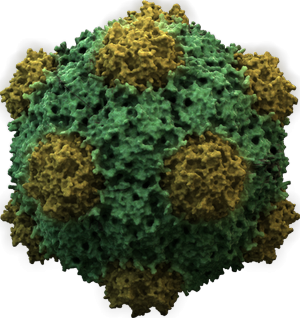
\includegraphics[width=2cm]{virusborig.png}}\\\hline\hline
Beschreibung:	& Viren sind vom Gegner kontrollierte\\
			& Einheiten. Sie besitzen die\\
			& Eigenschaft Stamm welche sie einem\\
			& Stamm zuordnet. Sie k\"onnen\\
			& keine Zellteilung betreiben, ebenso\\
			& nicht auf normalem Wege angreifen.\\
			& Viren sind in der Lage Einheiten des\\
			& Spielers sowie rote Blutk\"orperchen\\
			& zu befallen. Dabei dringen sie in diese\\
			& ein und verweilen dort w\"ahrend sie\\
			& weitere Virus Einheiten produzieren können.\\
			& Diese \"ubernehmen die Stamm\\
			& Eigenschafft des produzierenden Virus.\\
			& Dem Virus kann es \"uber Mutation\\
			& m\"oglich sein ungesehen in anderen\\
			& Einheiten zu verweilen.\\
			& Die Angriffsst\"arke des Virus und\\
			& die Virenresistenz einer Einheit spielen\\
			& eine maßgebliche Rolle f\"ur die Zellinfektion\\
			& durch einen Virus. Die Teilungsgeschwindigkeit\\
			& des Virus gibt an wie schnell er sich nach\\
			& einer Infektion verbreiten kann.\\
			& Die Angriffsst\"arke von Viren gegen\\
			& andere Zellen ist je nach Zellenart\\
			& unterschiedlich  und kann\\
			& \"uber Mutation spezialisiert werden.\\\hline
Lebenspunkte	& 4\\\hline
Angriffsst\"arke	& 3\\\hline
Lebensdauer		& 4\\\hline
Geschwindigkeit	& 4\\\hline
Teilungsgeschwindigkeit	& 4\\\hline
\multicolumn{2}{c}{}\\
\multicolumn{2}{c}{\textit{\large{Einheitentabelle}}}\\
\end{tabular}

\subsubsection{Sonstige Objekte}
\begin{description}
\item[Blutbahn]\hfill \\
\begin{center}
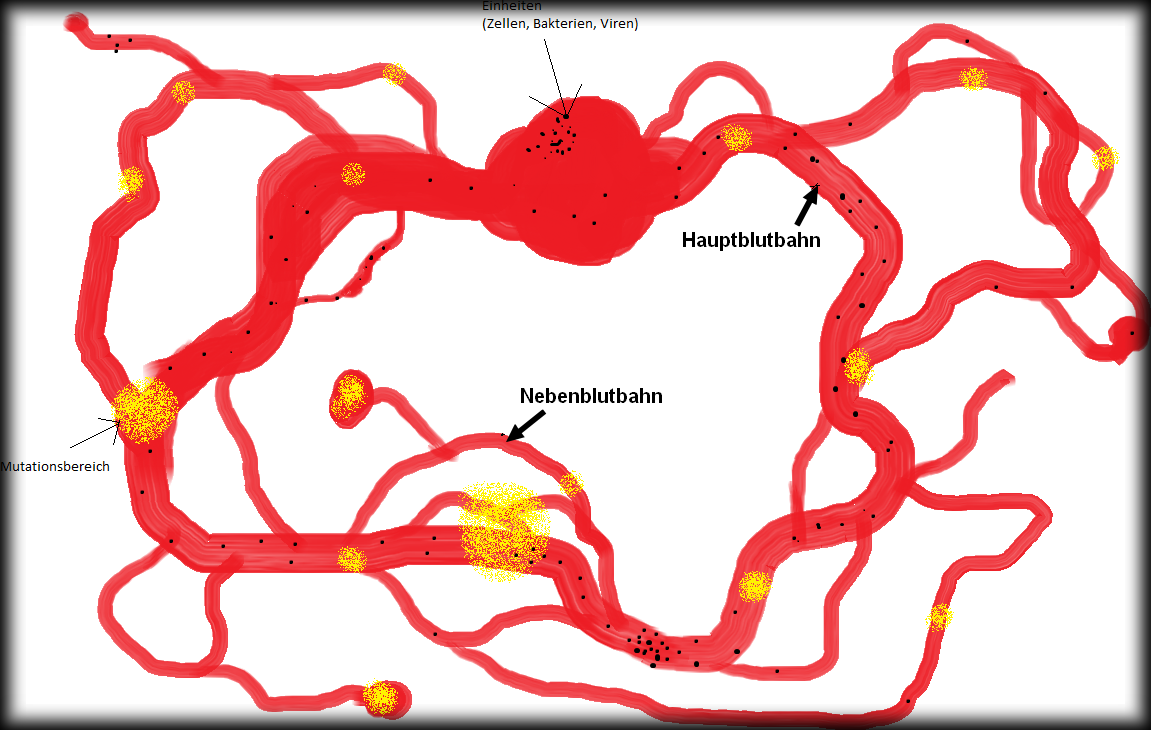
\includegraphics[width=10cm]{blutbahn.png}\\
\end{center}
Blutbahnen sind die begehbare Bereiche der Spielkarte. Es gibt Haupt- und Nebenblutbahnen die sich im Wesentlichen durch ihre Gr\"oße und Breite auszeichnen. Ist eine Einheit auf einer Hauptblutbahn kann sie sich dort schneller fortbewegen als auf einer Nebenblutbahn. Ebenso bewegen sich mehr rote Blutk\"orperchen (siehe \textit{Einheitentabelle}) auf Haupt- als auf Nebenblutbahnen. Blutbahnen haben eine Bewegungsrichtung, bewegt eine Einheit sich gegen diese Richtung wird sie langsamer. Dieser Effekt wirkt sich auf Hauptblutbahnen st\"arker als auf Nebenblutbahnen aus. Einheiten k\"onnen sich in dieser Bewegungsrichtung auf einer Blutbahn treiben lassen oder auf ihr ohne Bewegung stehen bleiben (siehe \textit{Optionen \& Aktionen}).

\item[Mutationsfelder]\hfill \\
\begin{center}
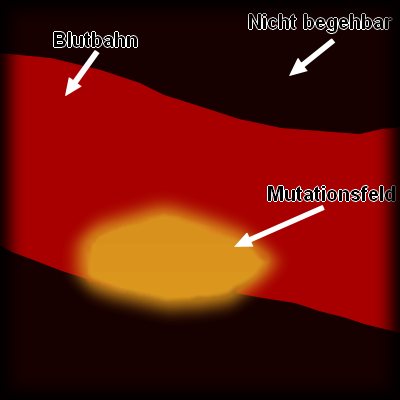
\includegraphics[width=5cm]{mutationsfeld.png}\\
\end{center}
Mutationsfelder sind zuf\"allige, auf Blutbahnen verteilte, persisente, begehbare Bereiche. Wendet eine Einheit w\"ahrend sie auf einem solchen Feld steht Zellteilung an ver\"andern sich die Werte der dadurch prodzierten Einheiten, welche sonst nur die selben Werte wie die urspr\"ungliche Einheit h\"atten. Dies trifft auch auf die speziellen Eigenschaftswerte einer B-Zelle (siehe \textit{Einheitentabelle}) zu, welche damit die Wirkung von Antik\"orpern bestimmt. Die Chancenverteilung ob die Einheit insgesamt verbessert oder verschlechtert wird h\"angt dabei maßgebend von der Gesamtwertung ihrer Eigenschaftswerte ab. Ist sie bereits stark ist es wahrscheinlicher, dass die Einheit insgesamt schlechter wird bzw. ist sie schwach wird sie wahrscheinlich verbessert. Mutationsfelder priorisieren zudem bestimmte Eigenschaften bei der Werte\"anderung, z.B. gibt es Felder welche bei \"Anderungen priorisiert den Wert Angriffsst\"arke \"andern. Bei der Zellteilung auf Mutationsfeldern geschieht es deutlich h\"aufiger, dass sich der Stamm einer Einheit \"andert (siehe \textit{Eigenschaftstabelle}).
\end{description}

\end{document}
